\documentclass[a4papert,11pt,notitlepage]{ltxdoc}
\usepackage[left=1.0in, right=1.0in, top=1.0in, bottom=1.0in]{geometry}
\usepackage[parfill]{parskip}
\usepackage{graphicx}
\usepackage{epstopdf}
\usepackage{mdwlist}
\usepackage{amssymb}
\usepackage{todonotes}
\usepackage{longtable}

\DeclareGraphicsRule{.tif}{png}{.png}{`convert #1 `dirname #1`/`basename #1 .tif`.png}
\bibliographystyle{plain-annote}

\title{Developing a device-agnostic, real-time ARS/PRS system with support for
broadcasting rich interactive content}

\begin{document}
\begin{center}
\textsc{\Large Final Major Project - Internet Engineering (H622)}\\[0.3cm]
{\Large \bfseries Developing a device-agnostic, real-time ARS/PRS system with support for
broadcasting rich interactive content}\\[0.3cm]
{\Large Progress Report}\\[0.3cm]
\emph{Author:} Thomas \textsc{Usher} \hspace{1cm} \emph{Supervisor:} Dave \textsc{Price}\\
\emph{Date:} October 3, 2010 \hspace{1cm} \emph{Version:} 1.0
\end{center}
\tableofcontents

\section{Project Summary}
\subsection{Introduction}
Audience Response Systems (ARS), more commonly referred to as 'clickers' have been used with varying degrees of success in educational establishments around the world for numerous years. Their use as a means to improve interactivity between students and instructors in an educational environment has been widely documented, with research indicating notable effects on student responsiveness, involvement and success. While this project will not involve additional research in to the value of PRS systems, it will attempt to highlight and enhance upon ``The give-and-take atmosphere encouraged by use of clickers which... makes the students more responsive in general''\cite{wood:clickers}.

From using these clickers from a students' perspective, I have noted two primary issues with the current implementation of these ARS systems:
\begin{itemize}
\item The devices are limited in what can be displayed on an individual users' device - while the majority have no displays at all, those that do typically only show which number/letter the user has selected. This limitation restricts interaction to simple question and answer style communication, as well as limiting potential for individual or group specific broadcasts.
\item Specific clicker hardware is required. While they can be relatively cheap, costs do increase with complexity and they are single-purposes devices. In most cases, specialist receiver hardware is also required and in larger scale cases, technicians are required to maintain these systems.
\end{itemize}

This project will attempt to solve the above issues by creating a 'next-generation' ARS system for use on any system with a relatively modern web-browser and the ability to access the local network. While the system should be platform and device agnostic, the increasing popularity of Apple's iPad and other tablet computers to enhance textbooks in education provides an ideal device around which to build and test the system within the time constraints (although it should not use any tablet or device specific implementations).

Clickers exist to improve interactivity during lectures, helping to engage students in the subject, improve attention-span and providing additional ways for students to feel personally involved in the subject. Secondarily, facilitating real-time feedback allows lecturers to tailor their approach based on the class response - for example, the lecturer might broadcast a set of questions about the current topic, if a large percentage of students answer incorrectly, the lecturer might wish to attempt another explanation. This project should maintain all of these benefits while building on the types of content which can be broadcast, as well as adding additional forms of interactivity where possible.

The system should be built around an extensible framework; allowing additional types of content to be created for broadcast, and to allow the system to be used in other use cases, such as school classrooms and business meetings. 

\subsection{Reasons for Project Choice}
Throughout my education I have been interested in ways to enhance learning through technology and interactivity. I often envisioned how a ARS might work before I first used clicker technology in my first year at Aberystwyth University, and after I'd used them, have since been thinking about how they can be improved, and how we can further real-time interactive education. 

I have personally noted a significant increase in responsiveness and interest shown by fellow students when clickers have been used in lectures, noting that others seem to pay more attention when interactivity is introduced as opposed to when they are being 'talked at' and that post-lecture discussion is more oriented around lecture material when clickers were used.

Unfortunately, it is a relatively uncommon occurrence to see these clickers being used, while almost every student tends to have a laptop, tablet computer or smartphone in front of them. There have also been numerous reports of educational departments supplying all of their students with iPads or laptops. I envision that developing a ARS system which works on these more common devices will encourage more frequent usage of this type of interactivity.

The technical challenges in this project were also interesting to me; I would need to facilitate real-time asynchronous communication to hundreds of devices at a time, work out how best to transfer and structure data for transfer and develop a means to collect and collate data returned from users' devices.

\section{Background}
Developing an effective system requires extensive research in to existing ARS solutions, devices which need to be supported, and technologies to be used in developing the project.

\subsection{Existing ARS Solutions}
A quick Google search for 'Audience Response System' quickly reveals the extent of the ARS market, with many companies producing their own specific hardware and software implementations. While the majority of products available are similar, I will take a more detailed look at a few.

\subsubsection{Qwizdom}
Qwizdom\cite{qwizdom:web} is the ARS system used by the Computer Science department at Aberystwyth University and is therefore the only one with which I have any direct experience. They provide two hardware solutions for learners:
\begin{itemize}
\item A keypad with a small E-ink display which shows the currently selected answer (the units currently used by Aberystwyth University are older versions of these units with an LCD display).
\item A keypad with a larger LCD display with the ability to display the current question and answers.
\end{itemize}

These interact via RF to a unit attached to a computer. The computer needs to be running ActionPoint, a PowerPoint/Keynote plugin which instructors can use to integrate questions in to their slideshows. When an ActionPoint slide is being displayed during a lecture, students' can submit answers to the question which is then immediately updated in ActionPoint. The lecturer can choose to display a graph of responses which can be reacted on immediately, or saved for reporting.

Qwizdom also supplies additional hardware for instructors to interact with their slides, including a tablet-style device.

This keypad style of ARS seems to be the most basic, tried and tested implementation, with other companies providing similar solutions to Qwizdom include; KEEPad, ShowMode, Votech, Group Dynamics and PowerCom, all of which do not offer anything beyond this type of interaction.

The issues with this keypad-style are what I noted in the introduction of this report; limited displays and the requirement for dedicated hardware. The integration with PowerPoint seems to be a good way of encouraging the use of these devices as a supplement to existing slideshow-based teaching, but I feel it makes the interactivity too oriented around slides where they could easily exist as separate entities if the device could display more information.

\subsubsection{IML, Genee World}
IML\cite{iml:web} and Genee World\cite{genee:web} are companies which both provide standard keypad based ARS', but have additional systems which are more in line with what I am trying to achieve with my project.

``IML enotes'' is a product focused on group meetings; allowing users on laptops to type feedback on a discussion topic and submit them anonymously over wi-fi to a central computer where they can be collated. The use of laptops is interesting but it appears to require specific software, laptops rented from IML, and an 'IML producer' to be present during the meeting. All of which seem very restrictive.

Genee World provide their ``Virtual G Pad'' solution; a web-based interface which appears to be emulating a keypad, interacting with the same server software (ClassComm) as their hardware based systems. The system can be accessed from modern browsers and should therefore run on tablets, phones and laptops, although the former two are not mentioned anywhere in the product description. As this system can run alongside their hardware, it is limited in the same ways.

The use of a web-based interface for the ``Virtual G Pad'' seems like an excellent way to ensure cross-device and multi-platform compatibility, definitely something to consider when planning my system.

\subsubsection{TurningPoint ResponseWare}
Again, TurningPoint\cite{responseware:web} offer hardware keypad solutions, but now have their ``ResponseWare Web'' solution. Similar to the ``Virtual G Pad'', this is primarily a web-based interface but it seems device specific applications for iPhone, BlackBerry and Windows Mobile devices are available. The website does not mention whether these applications are required to use this system on these devices or whether the web-based interface will adjust to be used on a touch-based device. There is also no mention of tablet devices or the Android mobile operating system.

The system runs over Wi-Fi or a mobile data connection - as it is likely that the majority of educational establishments to which this system is targeted are likely to have an established wireless infrastructure there would be no additional hardware or configuration required. This method of communication seems appropriate for the hardware independent solution I am working towards.

The main notable limitation in the ResponseWare system are the limited content types which can be broadcast, restricted only to simple Q\&A style content. In an improved system, the larger, more detailed screens on modern devices could be used to display a variety of rich content.

\subsubsection{Summary}
From researching existing ARS solutions, I have noted how these systems have evolved from simple keypads, through to web-based clients which can be used on modern mobile phones. Despite the software and hardware evolving, the companies I researched have not extended their solutions beyond basic Q\&A interactions, possibly due to the need to support legacy devices in their software. To create an ARS system which sets itself apart from the Virtual G Pad or ResponseWare, I will need to support additional types of rich content, such as images, websites, and interactive activities.

Existing solutions have also provided me with some suggestions as to how to build my implementation; particularly the use of a web-based interface rather than an application for every device I want to support, and the use of Wi-Fi/Data over HTTP for communication with the server.

\subsection{Devices and Operating Systems}
\label{sec:devices}
While the goal of my project is to develop a device/OS agnostic system, all the devices supported will need to be able to facilitate running the features required in an ARS with rich content support. This means they all need:
\begin{itemize}
\item A way to connect to a network, either over a cable, wi-fi or data connection (3G).
\item A reasonably sized colour screen - for the purposes of displaying rich content, an initial suggestion of a minimum resolution of 480 x 320 seems reasonable.
\item A flexible input mechanism; either touch or a pointing device and keyboard.
\item Some way of executing code/applications.
\end{itemize}

I will take a closer look at common platforms, devices and operating systems which meet these requirements in order to find a common set of features on which to build the project. Ideally, the system should use a minimal amount of device-specific code and should any be required, it should be easily changed without needing to re-deploy to client devices.

\subsubsection{Mobile Operating Systems}
First, I look at mobile operating systems. To determine what were the most popular mobile OS', I used an analysis of the smartphone market published in May 2010 by Gartner Inc.\cite{gartner:mobile}:

\begin{tabular}{l l}
Company & Market Share 2010 Q1(\%) \\
\hline
Symbian & 44.3 \\
BlackBerry OS & 19.4 \\
iPhone OS & 15.4 \\
Android & 9.6 \\
Microsoft Windows Mobile & 6.8 \\
Linux & 3.7 \\
Other OSs & 0.7 \\
\end{tabular}

I will take a more detailed look at all listed OSs with a market share of 5\% or larger. 

\begin{description}
\item[Symbian] \hfill \\
Symbian\cite{symbian:web}, the most popular mobile operating system has gone through many iterations since its original release as Symbian OS 6.0 in 2001 and is now found in all Nokia phones, as well as various mobile devices from Sony Ericsson, Sharp and Samsung.

The majority of Symbian devices are basic mobile phones which do not meet the necessary specifications (particularly a lack of a 3G data connection and large screen), but newer Nokia devices running Symbian OS 9.1 and later seem to be suitable, so this is the version of the operating system which I would likely need to target.

Software can be written for Symbian in various languages, primarily C++ with Qt but including Python, Java ME, Ruby and .NET. Developing a UI however, would need to use Symbian specific APIs, something which I would like to avoid. Device security is also left up to the vendor, meaning most devices can not run custom code, or only code approved by the vendor (such as through Nokia's Ovi store).

While various browsers are available for Symbian devices, they typically use the built-in browser supplied by the vendor. In Nokia's case, the Nokia Browser in Series 60 devices and above is built upon Apple's WebKit project\cite{nokia:browser}, particularly the WebCore and JavaScriptCore components - suggesting that the majority of newer Symbian devices use relatively modern browser components, including support for JavaScript. Some later versions of Symbian on Nokia devices can make use of Flash, Silverlight and JavaFX.

\item[BlackBerry OS] \hfill \\
RIM develops the BlackBerry\cite{blackberry:web} line of business smartphone devices, all of which run on BlackBerry OS. Most recent BlackBerry devices meet all the specifications listed above.

BlackBerry OS applications are typically written in Java using a set of APIs to interface with the operating system - this suggests a lot of device specific-code, so this approach is unlikely to be suitable.

As of BlackBerry OS 6, the bundled browser is also based on WebKit\cite{rim:browser}, and therefore supports modern web features and JavaScript. Later versions of BlackBerry OS also support Flash content, with plans to support Silverlight

\item[iPhone OS] \hfill \\
iPhone OS\cite{ios:web}, now known as iOS is Apple's mobile operating system which runs on all mobile devices built by Apple; iPod touch, iPhone \& iPad. 

Applications are built using the iOS SDK and written in Objective-C. They can only be distributed through the Apple Store, which requires approval from Apple and a fee to be a member of the iOS Developer Program. Again, as this requires device independent code in an entirely different language from the OS' I've researched so far, it doesn't seem like a suitable solution.

The browser on iOS is a version of Apple's Safari, also based on WebKit (Apple being the founder of and contributor to the project). iOS does not allow any third-party modifications to the operating system and built-in applications, so browser extensions such as Flash, JavaFX and Silverlight can not be used.

\item[Android] \hfill \\
Android\cite{android:web} is Google's open source mobile operating system licensed under the Apache License, allowing vendors to freely use and extend the OS, and as a result, it has been widely adopted by multiple manufacturers since its initial release.

Applications are typically written using Java and the Android SDK, although due to the open nature of the operating system, most languages can be used. Applications can either be distributed through a store, such as the Android Store bundled with the majority of phones, through a vendor-specific store, or transferred directly to the phone. While the flexibility of this platform could mean only a thin UI layer would need to be written for it, it would still require quite a significant amount of device-specific code to do so.

The bundled browser on Android devices is also based on WebKit, using Google's V8 engine for fast JavaScript execution. The browser can also be extended to use many web application platforms including Flash, Silverlight and potentially JavaFX (although there is no implementation currently available).

\item[Windows Mobile] \hfill \\
Microsoft's mobile OS, Windows Mobile\cite{winmo:web} has been used on various mobile devices built by a number of the world's largest mobile manufacturers. It is now being phased out in favour of the recently released Windows Phone 7.

Developing for Windows Mobile requires the use of Visual C++, or code on the .NET Compact Framework - more device independent code.

The Windows Mobile browser has had seen many iterations, although they are all based on Internet Explorer and therefore support most modern features and JavaScript. While JavaFX and Silverlight are supported on later versions of the platform, Flash support is not available.

{\it{\bf Note regarding Windows Phone 7:} For the purpose of this assignment, as it was released less than two weeks before this report was written, market share figures are not yet available, and based on initial reviews of the operating system, we will assume that Windows Phone 7 has a significant enough market share to be considered, and that it has feature parity with iOS, namely restrictions on custom applications and a modern browser.}

\item[Other] \hfill \\
There are a number of mobile operating systems which do not currently have a market share above 5\%, either because they have not yet been widely adopted, or because they have only recently been released. These include Nokia's Maemo (based on Debian), Blackberry's upcoming QNX-based Blackberry Tablet OS, and Palm's webOS. While I will not specifically research the applicability of these devices, I am confident that as the majority are either Unix-based, or released within the past two years, they all have a relatively modern web browser.

\end{description}

\subsubsection{PC Operating Systems}
Ensuring support for popular personal computer operating systems should not be as significant a task as supporting mobile operating systems. New innovations and technologies are almost always first implemented on PC OS' before eventually making their way to mobile devices, a transition which can take many years due to limited or differing hardware and alternative UI paradigms used on mobiles. PC OS' also tend not to be as restrictive as to what software can be compiled on them, usually down to compilers being available for most popular processor architectures.

For this reason; I will consider the three largest PC operating systems to be suitable for running this system, those three being Windows, Mac OS and Linux. Although all three come in various versions and incarnations, we can assume that given sufficient hardware, they can run any required code.

\section{Goals and Objectives}
\subsection{Outline System Requirements}
An initial list of system requirements which will be elaborated on in a full system requirements document, to be presented with the final report.

\subsubsection{Presenter}
\begin{itemize}
\item Presenters should be able to create and edit content using an easy-to-use interface.
\item A set of rich content-types should be made available for creation; including images, websites and QAs.
\item The presenter interface should facilitate the creation of 'plans', consisting of a set of content which can be broadcast to a certain audience.
\item Presenters should be able to specify what users are authorised to access plans.
\item A presenter should be able to push any created content to the audience through this interface.
\item Responses from the audience should be visible in this interface.
\item Types of content available for creation should be extensible without having to change any core components.
\item Authorisiation should be required to access the presenter interface.
\end{itemize}
\subsubsection{Client}
\begin{itemize}
\item Users should receive broadcast content within 5 seconds of the push.
\item Users should be able to interact with any interactive content, such as QAs.
\item The client system should be accessible on any device which meets the specifications in section \ref{sec:devices}.
\item The client should be not need to be updated when additional content types are added or changes are made to the presenter system.
\item A user will have to sign in and enter the ID of a plan which they are authorised to access before content is displayed.
\item A user should remain signed in for the duration of the session.
\item The history of content broadcast to the user during the session should be freely navigable using the client, even when a new piece of content has been broadcast to them.
\end{itemize}

\subsection{Example usage}
An example of how this system would work:
\begin{enumerate}
\item A lecturer would use the tools provided to construct a set of interactive slides before a lecture.
\item During the lecture, all students would access a certain URL in their tablet's browser.
\item The lecturer would choose to broadcast a certain interactive slide to all students when necessary.
\item All students' user agents would instantly update with the content.
\item If the slide is interactive, the lecturer would immediately receive notifications and statistics when a student responds.
\end{enumerate}

\subsection{System Limitations}
Although I would like this system to be as flexible as possible, I have identified limitations necessary to keep development time within the allotted period:
\begin{itemize}
\item The client systems' layout will only be designed to run on the iPad's screen size. While the system will work on any other specified device, creating layouts for other screen size will only be done if there is additional time available.
\item The system requires both the client and presenter to be on the same network.
\item Users will be unable to access content from past sessions.
\item Response to content will only be visible for the duration of the session.
\item Integration with PowerPoint slideshows such as with existing ARS systems will not be possible.
\end{itemize}

\section{Process Model}
For this project, I wanted to enjoy the development of the system as much as possible, so adopting a process model that best suited the way I write software was important to me. As my typical development methodology is 'hack at it until it works', I wanted to find a process that injected a degree of organisation in to the process, giving me a way to plan and view my progress while maintaining focus on the code rather than the documentation.

\subsection{Waterfall Model}
The 'traditional' methodology for software development goes through five steps, each of which must be completed before the project can progress to the next:
\begin{enumerate}
\item Requirements - A software requirement specification is produced, outlining all the requirements for the system.
\item Design - A design specification is created which details how all elements of the system will be designed and how they interact.
\item Implementation - The stage where the software is built to the design specification.
\item Verification - Ensuring the system meets the requirements.
\item Maintenance - Correct issues and ensure the system continues to run as required.
\end{enumerate}

This process would allow me to concentrate on the code once I reached the implementation stage, but it does require a lot of planning to begin with. It would also require me to have a very clear design before I even wrote a line of code without much of a chance to change that design during development. For example; I would prefer to be able to experiment with the server side of the project before I make a final decision on the design for other dependant parts such as the client.

\subsection{Test Driven Development}
TDD is very different to the waterfall model in that there is very little documentation required and the entire development process is built around the code.

Development consists of a rapid cycle:
\begin{enumerate}
\item Test written - every new feature begins with a test.
\item Run tests - ensuring the new test fails meaning the test is valid and that the feature is currently not implemented.
\item Write code - the simplest possible code that will pass the tst is written.
\item Run tests - ensure the new test now passes.
\item Refactor code - tidy the code on every iteration, ensuring the test still pass after refactoring.
\end{enumerate}
This process is repeated until all features are implemented.

I feel that TDD, while highly oriented around the code, would be unsuitable for my individual development style as it would prevent me from experimenting with the technologies I use. This project is also highly dependent on network communications between multiple systems written in different languages, writing tests for this type of interaction would likely overcomplicate the implementation.

\subsection{Iterative and incremental development}
Iterative development is a compromise between the well-planned approach of the waterfall model and the rapid iterations of TDD. Requirements are established at the beginning of the project and then separated in to iterations, usually based on their importance. Iterations are then implemented, integrated and then tested, at which point progress can be evaluated and the next iteration can be adjusted as required. Iterations continue until the system is complete (or time runs out).

This process seems more oriented around the way I develop; building a set of features before moving on to the next set of features. It provides the discipline and development periods focused on code found in the waterfall model while allowing the product to feed back in to the design as in TDD without hindering the experimentation of development.

As the system being built is divided in to its own distinct components, dividing them in to iterations not only makes sense from a planning perspective, but would encourage me to remain focused on individual parts of the system as I build them. The process also lends itself to the style of the project, in that the implementation of the server system (such as data interchange format, etc.) can feed back in to the plan for the client.

\subsection{Conclusion}
I have concluded that the most appropriate development methodology of those that I have researched is iterative development. I feel it best suits how I build software, allowing me blocks of time in which I can focus on writing code, while adding a sense of organisation and planning to the process. While the waterfall model might also have been suitable, I considered the requirement to complete the design before moving on to development too restrictive as I believe any software project needs room to evolve during its implementation.

\subsection{System Evaluation and Testing}
Using an iterative development process will allow me to thoroughly test the system at various stages throughout its development. 

As I know the requirements of my system, I will develop a requirement specification, break down requirements in to iterations and develop test plans for each iteration. Between each iteration, I will execute its test plan, integrate the system and revise the plans for the next iteration as required. At the end of development, I will re-execute all test plans to ensure all requirements are still met.

\section{Technical Challenges}
\subsection{Multiple Device Support}
One of the main goals of this system is to have the client usable on a wide range of computing devices. My extensive research in to these devices in section \ref{sec:devices} shows that there is very little crossover in language support between platforms. I could potentially write a core library in C and integrate that in to device specific applications, but that would mean writing many applications to cover as many platforms as possible - it would also require a lot of maintenance in the future when new platforms or updates required support.

A common solution for writing cross-platform applications is to use a web-based interface; from my research the majority of the targetted devices support a modern web browser, typically based on WebKit. Writing a web application should give me the cross-platform support I need without requiring any device specific code, short of some per-platform optimisations and layouts for different screen sizes. This does mean I will lose some of the flexibility of a device-native application - I will have to emulate a rich, interactive user interface using HTML, JavaScript and CSS, rather than any built-in APIs provided by the device.

As I do not have access to the majority of these devices and optimizing the UI for different screen sizes would be a time consuming process, I will likely only attempt to create a UI for the screen size of the Apple iPad, ensuring that there is no device specific code and that creating layouts for different screen sizes requires no more than the addition of a CSS file. Should time allow, I will also create a layout for smaller mobile phone screens, such as the iPhone.

\subsection{Real-Time Communication}
As this application requires content to appear on all client devices within a reasonable period of time after they are broadcast, it will need to use some form of real-time communication method. As it seems likely that the only possible multi-platform solution is to use a web-based system, this makes this requirement much more complicated as the HTTP protocol is entirely request-response oriented. If I was using code which was not being executed in the browser, I could use networking technologies such as sockets to allow the client to 'listen' for communication from the broadcaster.

However, there are various ways to support a  communication channel in web applications, WebSockets (from the HTML5 specification) and Flash Sockets being the most direct solutions although unfortunately they are not yet implemented or available in the large majority of browsers, particularly those on mobile devices. Sockets can also be emulated using techniques such as long polling or multipart streaming. Working out which of these of these techniques to use, learning the protocol and writing an implementation which can fallback to another if required will be a complicated part of this project. Ideally, I will be able to find a library for whatever server-side implementation I use which does the majority of this work for me.

As real-time communication is one of the primary features of an ARS, this whole project hinges around this being successful. While I am confident that it is feasible due to experience in building real-time web applications in the past, I will fall back to a simple request-response architecture for content if absolutely necessary, requiring users to click a button to 'request' the next item from the server.

\subsection{Traffic Bottlenecking/Performance}
\label{sec:performance}
My concern with broadcasting content in real-time to hundreds of devices at a time using a typical web server is that it is likely to struggle with the number of requests. Techniques used to emulate real-time communication either require a permanent connection open to the server, or hundreds of requests to the server per minute. Traditional web servers such as Apache use a process-based model, where each additional request requires a new thread meaning many hundreds of connections being opened and closed per minute not only causes high memory usage, but incurs quite a large processing overhead, increasing the time it takes to serve a request as the volume increases.

Event-based servers may be the solution to this issue which use a single thread and an event loop, removing the requirement for context switching. While this does mean significantly lower memory usage and overhead, it doesn't prevent operations in code from blocking, particularly those that involve I/O. For example; a request which queries the database will temporarily hold up the loop until the database responds, as we require a very quick response from the server, this may prove unacceptable.

To resolve this, I can tackle the problem on two fronts; reducing the amount of I/O time required through caching, and attempting to prevent I/O from blocking. Some libraries such as node.js provide an event-loop based language construct, allowing requests to provide a callback which is only executed when the response is returned, allowing the server to continue while waiting for a response. To cache, I could use any number of caching solutions such as an in-memory key-value store.

The requirement to be able to serve many request at a high-speed, while important to a large scale system, is not necessarily required for the system to work, so if this proves too much of a challenge I can safely fall back to a more standard server, such as Apache.

\section{Outline Design}
The current state of the system design is outlined in this section.

\subsection{Use Cases}
There are two user roles for this ARS system;
\begin{itemize}
\item Presenter - users who will be presenting lessons/meetings - typically a lecturer or teacher.
\item Audience - users with client devices who will be receiving broadcasted content - typically students or meeting attendees.
\end{itemize}

Both roles will have different abilities on the system although the audience role is a subset of the presenter role, meaning a presenter can perform all actions on the system. In some cases, additional authorisation is required for certain actions, as noted below.

\begin{tabular}{l l l}
Task & Presenter & Audience \\
\hline
Access presenter system & \checkmark &  \\
Access client system & \checkmark & \checkmark \\
Create content & \checkmark & \\
Create plans & \checkmark & \\
Edit content & \checkmark if owner & \\
Edit plans & \checkmark if owner & \\
Delete content & \checkmark if owner & \\
Delete plans & \checkmark if owner & \\
Set plan permissions & \checkmark if owner & \\
Push content for broadcast & \checkmark & \\
Access plan from client & \checkmark & \checkmark if authorised \\
Receive broadcast content & \checkmark & \checkmark if authorised \\
Respond to content from client & \checkmark & \checkmark if authorised \\
View responses on presenter system & \checkmark & \\
View plan history & \checkmark & \checkmark if authorised \\
\end{tabular}

Figure \ref{fig:usecase} shows a use case diagram of interactions with the system.
\begin{figure}[htb]
\begin{center}
\leavevmode
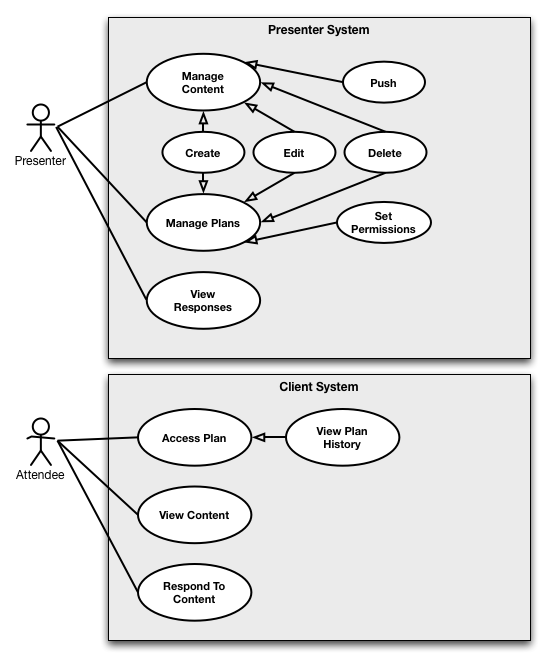
\includegraphics[width=0.7\textwidth]{use-case}
\end{center}
\caption{Use Case Diagram}
\label{fig:usecase}
\end{figure}

\subsection{System Tasks}
\subsubsection{Authorisation}
On initially accessing either the presenter system, the user is in an unauthorised state and therefore unable to view any content. They are prompted to enter user credentials and on doing so, the system validates their permissions to ensure they have the presenter role. Once they are validated, the user enters an authorised state and they can view, create and edit content. If their credentials are invalid or they do not have the correct role, an error is displayed and they are returned to the login UI.

On accessing the client, the user is prompted to enter their login credentials. Once verified, they enter an authorised state and are then prompted to enter a plan ID - this is the identifier for the 'lesson' created by the presenter. Once entered, the users' ID is checked against the authorised users for the plan - if they are authorised to access it, then the plan is displayed.

\subsubsection{Presenter Content Management}
An authorised user with the presenter role can manage content and plans using the presenter system. On initiating the creation of the required content type, the presenter is given a set of fields to complete, once completed, clicking a button creates the content and adds it to the list of all content.

Selecting the 'edit' option next to a content item from the list of all content takes the user to a set of fields pre-populated with the existing values for the content, they can then make any changes required and click a button to save the changes.

On pressing a 'delete' button next to the content item in a list, the user is prompted for confirmation of the operation and on confirmining, the content item is deleted.

Plans (a set of content items) can be managed in a similar way. Opting to create one gives the presenter a set of fields from which they can choose what content items to include in the plan. They also enter a list of users authorised to access the plan. On clicking a button, the plan is saved.

Editing and deleting plans is done in the same way as with content items.

\subsubsection{Broadcasting Content}
To broadcast content to users, the presenter must be authorised and have a plan created with a set of content items. Each content item in the list has a 'Push' button next to it. On pressing this button, all users currently logged in and viewing this plan will see the content item on their client devices.

\subsubsection{Working with Content on the Client}
On authorisation and selection of a plan from the client system, the user is presented with an empty display until content is pushed from the plan by the presenter. There are no options for interaction with the content at this point.

Once new content is pushed to the client, it can be interacted with as specified by the content type. It is also made available in a 'history' of pushed content on the client, which can be navigated as required.

\section{Implementation Options and Choices}
\subsection{Client System}
Research in to mobile platforms indicate that there is very little similarity between development solutions for the majority of platforms. I will briefly look at my options for the client application and detail the option I have chosen.

\subsubsection{Common Library}
Although the majority of the systems I have studied require development in various languages and using device-specific APIs, it is likely that I could build a library in a low-level language such as C++ and create thin UI layers for each device. While this means I could take advantage of the benefits of each platform, it does have a number of disadvantages:
/begin{itemize}
/item Time required to create and maintain clients for each platform is prohibitive. It pushes the boundaries of the 'multi-platform' philosophy too far.
/item I am not proficient in C++ or C, learning these languages to the level required for implementation of these network protocols would take a lot of time.
/item This system uses many high-level ideas not suited for C/C++.
/end{itemize}

\subsubsection{Cross-Platform Languages}
Many devices that I studied support Java. As Java code runs in a virtual machine, there is a significant 'write once run anywhere' benefit with using Java. There would still be a requirement to write device-specific code to interface with their layout APIs. I have used Java extensively, so I would feel comfortable writing an application using it, but I would still need to learn a lot about mobile operating system APIs in order to ensure the system is flexible enough. Java is also not supported on iOS, one of the largest mobile operating systems and the one I use most myself.

\subsubsection{Rich Web Multimedia Platforms}
Rich web-based platforms such as Flash, Siverlight and JavaFX have implementations on multiple devices. With these platforms, everything from the operational code to the interface are entirely interprted by the platform. This would mean that writing, for example, a Flash-based solution once, would run on every platform which supports Flash without any additional code. Although I feel the idea behind these systems is good, I don't personally believe in requiring proprietary extensions to run the application and I can not find one of these platforms which is available across all platforms I have studied.

\subsubsection{Browser-Based}
Browsers are available on the vast majority of user agents in variatons incarnations - in my research I noted that every platform I studied had a proficient browser, most being based on the WebKit\cite{webkit:web} open source project (providing HTML rendering and JavaScript implementations) which is also used for Google's Chrome and Apple's Safari browsers. From past experience, I know how web applications can be used for excellent cross-platform support, backed up by research in to existing multi-platform ARS' systems, which all appear to be web-based.

A web-based client solution would be accessible from any device with a browser that supported full HTML, JavaScript and some form of real-time communication protocol (even if emulated), features which all of the devices I researched have. No device-specific code would be required, although styles for different screen sizes would be necessary. It would also be possible to use technologies only present in more modern browsers (such as HTML5 features) by making use of graceful degradation on devices that do not support it.

\subsubsection{Decision}
I will be using a browser-based solution for the client as I feel it is the most appropriate option for a truly multi-platform system. While I may lose some of the flexibility of device-native applications, this is an appropriate compromise. Past experience with web applications using JavaScript and an understanding of how to implement a real-time application also contribute to this decision.

The web application will be a thick client, with the majority of operations performed on the client, this means heavy use of JavaScript and HTML5 features where applicable. The client will connect to a server from which it can retreive content.

\subsection{Presenter System}
As the presenter system need only be executed on a presenters' computer and does not need to be multi-platform, I could potentially implement it in any language I choose. However, as the client will be web-based, I can reuse a lot of components as well as share resources such as templates if I also implement the presenter as a web-based system. It also means I can use the presenter web server as the server through which my client application can receive content.

I do need to choose what language I will implement the presenter web-system in, although as it is a relatively simple application which just needs to interface with the database, I don't believe the language choice is of particular importance. I could write it in Java, PHP, .NET, Ruby or Python and they would all perform similarly and provide similar libraries - the only factors on which I would select a language would be portability and my knowledge of it. As all of the listed languages are usable on Unix, OSX and Windows servers, I will be using a web development language with which I am most familiar, Python.

A web framework known as Django\cite{django:web} is available for Python which abstracts away many of the repetitive parts of building a web application; user authentication, databases (using it's own ORM) and templating, all of which are already provided when using Django. As I don't consider these aspects of the system to be a focal point of development in my system, I will be using Django so that I can spend more time concentrating on the important parts; real-time communication and the client.

The presenter system will also be using a relational database to maintain a persistent store of content and plans. As Django's ORM abstracts the database away and supports many systems, the choice of RDBMS is not as important as it would be if I were not using a framework, therefore I will use the RDBMS with which I am most familiar, MySQL.

\subsection{Real-Time Communication on the Server}
To facilitate fast real-time communication between client and server, I will need a server and language which allows such rapid communication (detailed in section \ref{sec:performance}). Here I will detail which solutions I looked at and my final decision.

\subsubsection{Thread based servers}
The simplest possible solution is to a thread based server (such as Apache) to host the system. This would work how most typical web applications work; on a new request, all clients connect to the Apache server and a thread is created for each client. If a message is pushed to 100 clients, all 100 clients simultaneously request a resource from the server, creating 100 threads which are closed as soon as these requests are complete\cite{nginxapache:web}. Some clients, due to real-time communication techniques such as long polling, will hold a connection open for the entire duration of their connection, permanently holding resources on the server. I don't believe this would be suitable for a real-time application and am therefore ruling out thread based servers altogether.

\subsubsection{Event based servers}
Event based servers (Nginx, for example), on receiving a request from the client adds the request to a queue, an event loop runs over the queue, processing the request and executing their callback, allowing requests to come in as other requests are being processed. This means that when a connection is inactive, no resources are being used and that there is significantly less overhead and memory required to handle a request. This leads to the ability to handle a significantly larger number of requests.

\subsubsection{Event-driven language frameworks}
Being able to handle many concurrent connections through the use of an event based server solves part of the problem, but there are still issues if the code being written is blocking (the main execution loop of the program must wait for an event to complete before it can return, holding up other processing). Event driven programming works in the same way as an event driven server - using a main event loop to support callbacks from functions so that operations can continue while I/O is being performed, operating on the results only when they return.

This type of programming paradigm is implementable in the majority of programming languages, although it is more prevalent and easier to implement in functional languages such as Erlang and Scala. There are also a number of frameworks for other languages available which support event-driven networking, such as Twisted (for Python), EventMachine (for Ruby) and Node.js (for JavaScript). 

As I am not familiar with functional languages, I will not be attempting to implement a server in Erlang or Scala, but the existing event-driven networking frameworks interest me as they do not require learning a new language and seem relatively popular. Twisted and EventMachine are mature frameworks, both with a large community and many extensions, but they both seem too bloated for what I need. Node.js is a relatively new framework which is rapidly gaining popularity, primarily because of its speed and simplicity - it interests me because it uses JavaScript which is also used by my client system (an opportunity for more code reuse and resource sharing) and is a language with which I'm familiar. There is also a library available for it which abstracts a lot of the client-side communication issues as I will detail in the next section.

\subsection{Real-Time Communication on the Client}
Web-based applications aren't usually known for taking advantage of real-time communication, it wasn't until the increased popularity of Ajax that we saw anything beyond standard request-response style websites. Even now, the most common type of interactions require the web browser to make a request to the server before it updates anything. However, we are now beginning to see 'comet'\cite{crane:comet} style web sites, where the client can 'listen' to a server, updating whenever something changes in applications such as chatting. This is made possible using various techniques which either create or emulate 'socket' style connections:
\begin{description}
\item[WebSockets] \hfill \\
An implementation of a communication channel over TCP for use implementation in web browsers as part of the W3C HTML5 specification. Currently only implemented in the latest version of modern browsers, excluding Internet Explorer.
\item[Flash Sockets] \hfill \\
TCP sockets can also be implemented using the ActionScript 3.0 Socket class, requiring the browser to load a Flash file and therefore requiring the Flash browser plugin. While this is the next best thing to using WebSockets, many mobile browsers do not fully support Flash.
\item[Ajax long polling] \hfill \\
A technique which is most commonly used for real-time web applications as it only requires a browser to support the XMLHttpRequest object, commonly used for Ajax interactions. This technique makes an asynchronous request to the server which the server keeps open until it has new data to send. As soon as new data has been received, the browser starts a new long polling request. While this technique is available on more devices, it is also slower and causes the browser to constantly be in a 'loading' state.
\item[Multipart streaming] \hfill \\
The XMLHttpRequest object can also be used to react to a server using a multipart content type; suggesting to the browser that the response will be delivered in multiple parts. The browser keeps the connection open and calls a callback function whenever a new part of the response is delivered.
\end{description}

There are other techniques, but the above are most commonly used. Unfortunately, the only one which reliably works on a large subset of browsers is long polling. I could implement the system using just this techniques, but it would then be unable to take advantage of the faster protocols such as WebSockets, available on the latest mobile browsers (such as Safari on iOS 4.2.1).

A library is available for Node.js, socket.io which allows both the client and server to determine which technique to be used and fall back to it as required, with an API to abstract these details away. This would allow me to support many different browsers with whatever technique they require without having to re-implement all the methods and is therefore what I will be using for this part of the system.

\subsection{Pushing Content to the Client}
To have content pushed from the presenter system to the client, I will need a way for one system to tell the other what content to broadcast and when. 

To begin with, it is necessary to figure out in what format I should be serialising data for transfer between all the systems involved. As both Python and JavaScript have native support for serialising to/from JSON (JavaScript Object Notation), a lightweight format designed for data transmitted between a server and web application, this seems like a natural fit for this project.

Sending the data from presenter to the node.js server could be done by sending it a POST request with the JSON as the value, which could then parse the object and determine which clients to send it to. The node.js server will then need to cache this object so that all future request for it from the client will not cause an additional request back to the presenter, leading back to the original bottlenecking problem.

It would be possible to simply have the distribution server store the JSON in memory, but if this system were serving tens of sets of audiences at a time, this caching implementation would best be suited to a tool designed for this type of use. Key-value databases are particularly useful at this type of task, allowing very quick retrieval of content by key from memory. Memcached is a commonly used implementation, but I have experience with Redis, a VMWare product which performs a similar task, has a very simple, clean interface and has libraries for both Django and Node.js.

Redis can also be used as a Publish/Subscribe server - allowing me to do away with the POST request by having Django publish the latest object ID to be broadcast directly to a pub/sub channel which the distribution server is subscribed to. On receiving an update from the channel, the node server can request the JSON object from the presenter server, cache it in Redis and then distribute it out to clients from the cached copy.

\subsection{Hosting}
As both the client and presenter system require a web server, I will need to configure one for development and testing. I could use a shared hosting provider, but as I'm using relatively complicated communication techniques and a language/framework not usually support on shared hosts, I will use a VPS provided by Linode. The VPS runs Ubuntu 10.04 and allows me full access to everything running on the server.

On the VPS I will configure Nginx to host my Django application, a Node.js server to run the distribution server and to server resources to the client, a MySQL database for the persistent storage of content and a Redis instance for caching and the publish/subscribe channel.

\subsection{Tools}
To develop the system I will use a private git repository with a remote set up on GitHub. A clone will be set up on any local development machine and on the server. I will either develop directly on the server through SSH, or modify a clone, push to the Git remote and then pull the updated copy on the server.

I will be using Vim as my editor as I will be developing over SSH for the majority of the time and I find it fast and powerful when coding.

\section{Project Plan}
My chosen process model, iterative development allows me to break down the project in to iterations so that I can inject an element of organisation in to my generally chaotic development process. As I am the client, I have chosen to use one iteration per system section, rather than implementing important features first. This will allow me to have a functional broadcast system by the third iteration from where I can feed back what I have developed in to the fourth iteration, for adding interactivity features, the fifth iteration, for additional features and the sixth iteration, for polishing the system.

I have not used a system to calculate how long each task will take, instead choosing to estimate based on experience of similar tasks. Instead, I have moved non-critical, 'nice to have' tasks to iteration 6. Should I have any unfinished tasks from iteration 1-5 to complete, I will do these in iteration 6 instead.
 
\subsection{Iteration Breakdown}
\begin{longtable}{l p{7cm} l}
Task & Description & Days \\
\hline
Iteration 0 & Initial Planning \& Configuration & 26-28th Nov \\
\hline
Produce project requirements & Create a document expanding on this list with project requirements, break them down in to iterations & 26-28th Nov  \\
Produce test plan & Create a test plan for each iteration to test whether requirements for that iteration have been met. Include integration tests and test for the complete system. & 26-28th Nov \\
Configure server & Install Nginx, Node.js, MySQL and Redis on VPS and configure as required & 28th Nov \\[1cm]
\hline
Iteration 1 & Presenter System & 29th Nov - 10th Dec \\
\hline
Content models & Create definitions for content models in the system & 30th Nov - 1st Dec \\
Administration interface & Develop basic interface for managing and creating content & 2-6th Dec \\
Serialisation system & Create system for serialising content objects in to JSON for transfer to the distribution server & 7th Dec \\
Authorisation system & Develop system for authorising presenter users & 8th Dec \\
Pushing content & Create interface with Redis pub/sub channel for pushing content as required & 9th Dec \\
Testing & Execute test plan, produce updated documents as required & 10th Dec \\[1cm]
\hline
Iteration 2 & Distribution Server & 11 - 18th Dec \\
\hline
Redis interface & Configure interface to Redis pub/sub channel for receiving updates & 11th Dec \\
Caching system & Use Redis for caching content to be broadcast & 11-13th Dec \\
Broadcast configuration & Use socket.io for broadcasting content to the required channels & 14-15th Dec \\
Content server & Enable client to connect to server for accessing resources for thick client & 16-17th Dec \\
Testing & Execute test plan, produce updated documents as required & 18th Dec \\[1cm]
\hline
Iteration 3 & Client System & 19 - 30th Dec \\
\hline
Authorisation & Enable users to authorise themselves to receive content & 19th Dec \\
Real-time connection & Use socket.io to listen to content from distribution server & 20th Dec \\
Templating system & Create system for parsing the JSON, fetching a template from the server and displaying the content as required & 21-23rd Dec \\
History & Create interface for navigating broadcast history on the client & 27-29th Dec \\
Testing & Execute test plan, produce updated documents as required & 30th Dec \\[1cm]
\hline
Iteration 4 & Interactivity & 1 - 13th Jan \\
\hline
Specify interactivity & Allow templates to specify how a user can interact with them & 1-3rd Jan \\
Serialise interactions & Create module for serialising interactions to JSON for returning to the server & 4-5th Jan \\
Distribute responses & Enable distribution server to return responses to presenter & 6-9th Jan \\
Parse responses & Enable presenter system to parse and store responses from content & 10-12th Jan \\
Testing & Execute test plan, produce updated documents as required & 13th Jan \\[1cm]
\hline
Iteration 5 & Additional Features & 14th Jan - 8th Feb \\
\hline
Add content types & Create new content types for broadcast & 14-17th Jan \\
Examination Period & & 17th-29th Jan \\
Improved presenter interface & Create Ajax-style interactions to improve content creation process & 30th Jan - 2nd Feb \\
Device independent client & Abstract device-specific code (CSS) on client away & 3rd Feb \\
Create iPad style & Develop CSS for laying out content on an iPad display & 4-7th Feb \\
Testing & Execute test plan, produce updated documents as required & 8th Feb \\[1cm]
\hline
Iteration 6 & Polish System & 9 - 18th Feb \\
\hline
Support other devices & Create additional CSS files to demo support on other devices & 9-11th Feb \\
Clean presenter interface & Tidy up presenter UI for ease of use & 12-13th Feb \\
Clean client interface & Tidy up client UI to ensure content is easy to see and interact with & 14-15th Feb \\
Add more content types & Add a content type which could be used in a different situation, such as a business meeting, for demonstration purposes & 16-17th Feb \\
Testing & Execute test plan, produce updated documents as required & 18th Feb \\[1cm]
\hline
Project Completion & Test, evaluate and write report & 19th Feb - 5th May \\
\hline
Testing & Thoroughly test system to test specification & 19-22nd Feb \\
Write dissertation & Write dissertation and supporting material & 23rd Feb - 5th May \\
\end{longtable}

\bibliography{bibliography}

\end{document}